\chapter{Introduction}

\begin{definitionii}
\textbf{\emph{dissertation}}
\textipa{[dis@\super rteiS\super @n]}
% dɪsəʳteɪʃən

\noindent   
A dissertation is a long formal piece of writing on a particular subject, especially for a university degree.

\noindent \emph{He is currently writing a dissertation on the Somali civil war.}

\hfill -- Collins English Dictionary \autocite{Smith1998}
\end{definitionii}

Above you will find a nicely typeset definition.
\lipsum[1-4]
\lipsum[1-4]

\begin{figure}
    \centering
    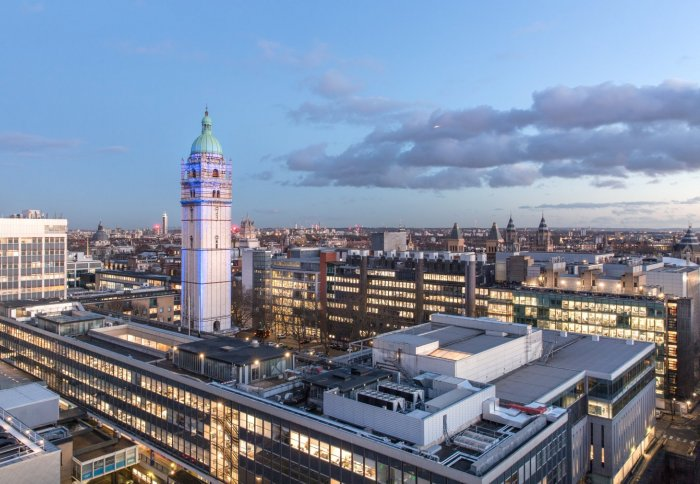
\includegraphics[width=0.8\textwidth]{img/imperial.jpg}
    \caption{Example of including an image}
    \label{fig:imperial-picture}
\end{figure}

\lipsum[2-4] See Figure \ref{fig:imperial-picture}.

\begin{table}[]
    \centering
    \begin{tabular}{llr}  
        \toprule
        \multicolumn{2}{c}{Item} \\
        \cmidrule(r){1-2}
        Animal    & Description & Price (\$) \\
        \midrule
        Gnat      & per gram    & 13.65      \\
                  &    each     & 0.01       \\
        Gnu       & stuffed     & 92.50      \\
        Emu       & stuffed     & 33.33      \\
        Armadillo & frozen      & 8.99       \\
        \bottomrule
    \end{tabular}
    \caption{Example booktabs table. Booktabs tables are nicer than regular ones, in my opinion. This site has a nice GUI for making LaTeX tables, and has a Booktabs option: https://www.tablesgenerator.com/}
    \label{tab:my_label}
\end{table}

\lipsum[1-4] Table \ref{tab:my_label}

\section{Section Example}
\lipsum[1]
\subsection{Subsection Example}
\label{subsection:example}
\lipsum[1]
\subsubsection{Subsubsection Example}

Note that you can reference chapters, sections, subsections and subsubsections. For example: Subsection \ref{subsection:example}

\section{Math Example}

\[
\textrm{score}(x) = \left(\lambda_m\sum_{i=0}^{|\mathbf{m}|} \log \hat{p}_m(d(x, \mathbf{m}_i) \mid l_i)\right) + \left(\lambda_l\sum_{i=0}^{|\mathbf{l}|} \log\hat{p}_l(d(x, \mathbf{l}_i) \mid \mathbf{v}_i)\right) + \lambda_p \hat{p}_p(x)
\]

\section{Algorithm Example}

See Algorithm \ref{algorithm:posit}

\begin{algorithm}[]
\SetAlgoLined
\SetKwInOut{KwInput}{Input}
\SetKwInOut{KwOutput}{Output}
\SetKwInOut{KwPre}{Pre}
\SetKw{Return}{return}
\SetKwProg{Fn}{Function}{}{end}
\LinesNumbered
\KwInput{$\textbf{m}$, such that $\mathbf{m}_i$ is the position of the $i$'th monitor\newline
$\textbf{l}$, such that $\mathbf{l}_i$ is the position of the $i$'th landmark\newline
$\mathbf{p}^m$, such that $\mathbf{p}^m_i$ is the ping latency from monitor $i$ to the target\newline
$\mathbf{p}^l$, such that $\mathbf{p}^l_i$ is the set of ping latencies to landmark $i$}

\BlankLine
\KwPre{Compute $\hat{p}_m(d \mid l)$, an estimator giving the likelihood of the target being distance $d$ away from the monitor, given that the monitor records a latency of $l$ to that target. Implemented by training a KDE using $\mathbf{p}^l$.\newline
Compute $\hat{p}_l(d \mid v)$, an estimator giving the likelihood of the target being distance $d$ away from the landmark, given a Canberra distance of $v$ between the target and the landmark, using training targets.
}
\BlankLine
\KwOutput{Most likely location of the target}
\BlankLine

\Fn{Likelihood($x$, $\mathbf{v}$)} {
MonitorScore $\gets \sum_{i=0}^{|\mathbf{m}|} \log{\hat{p}_m(d(x, \mathbf{m}_i) \mid l_i)}$\;
LandmarkScore $\gets \sum_{i=0}^{|\mathbf{l}|} \log{\hat{p}_l(d(x, \mathbf{l}_i) \mid \mathbf{v}_i)}$\;
\Return MonitorScore + LandmarkScore
}

\BlankLine
$\mathbf{v} \gets $\{$\mathrm{canberra\_distance}(\mathbf{l}_i, \mathbf{p}^m) \mid \mathbf{l}_i \in \mathbf{l}$\}

$\mathbf{C}$ $\gets$ Constraint-Based-Geolocation($\mathbf{m}$, $\mathbf{p}^m$)\;
$\mathbf{C_l}$ $\gets$ \{$m \in \mathbf{m} \mid \mathbf{C}$ contains $m\} \cup \{l \in \mathbf{l} \mid \mathbf{C}$ contains $l$\}\;
\BlankLine
\Return argmax$_{x\in \mathbf{C_l}}$ Likelihood($x$)

 \caption{Algorithm example}
 \label{algorithm:posit}
\end{algorithm}